\documentclass[tikz,border=8pt]{standalone}
% Shared look for every TikZ diagram. Load with % Shared look for every TikZ diagram. Load with % Shared look for every TikZ diagram. Load with \input{../../tools/tikz-style.tex}
\usepackage[T1]{fontenc}
\usepackage{lmodern}
\renewcommand{\sfdefault}{lmr}  % diagrams use the same serif as the text
\usetikzlibrary{arrows.meta, positioning, shapes.geometric, calc, fit, backgrounds}
\definecolor{cblue}{HTML}{4C78A8}
\definecolor{corange}{HTML}{F58518}
\definecolor{cgreen}{HTML}{54A24B}
\definecolor{cred}{HTML}{E45756}
\definecolor{cpurple}{HTML}{B279A2}
\definecolor{cgrey}{HTML}{6B6B6B}
\tikzset{
  every picture/.style={font=\sffamily, line width=1.2pt},
  box/.style={draw=#1, fill=#1!12, rounded corners=4pt, align=center, inner sep=7pt, minimum height=1.1cm},
  box/.default=cgrey,
  arrow/.style={-{Stealth[length=3mm]}, draw=cgrey, line width=1.4pt},
  title/.style={font=\sffamily\bfseries\Large},
  note/.style={font=\sffamily\small, text=cgrey, align=center},
}
\AtBeginDocument{\hyphenpenalty=10000 \exhyphenpenalty=10000}

\usepackage[T1]{fontenc}
\usepackage{lmodern}
\renewcommand{\sfdefault}{lmr}  % diagrams use the same serif as the text
\usetikzlibrary{arrows.meta, positioning, shapes.geometric, calc, fit, backgrounds}
\definecolor{cblue}{HTML}{4C78A8}
\definecolor{corange}{HTML}{F58518}
\definecolor{cgreen}{HTML}{54A24B}
\definecolor{cred}{HTML}{E45756}
\definecolor{cpurple}{HTML}{B279A2}
\definecolor{cgrey}{HTML}{6B6B6B}
\tikzset{
  every picture/.style={font=\sffamily, line width=1.2pt},
  box/.style={draw=#1, fill=#1!12, rounded corners=4pt, align=center, inner sep=7pt, minimum height=1.1cm},
  box/.default=cgrey,
  arrow/.style={-{Stealth[length=3mm]}, draw=cgrey, line width=1.4pt},
  title/.style={font=\sffamily\bfseries\Large},
  note/.style={font=\sffamily\small, text=cgrey, align=center},
}
\AtBeginDocument{\hyphenpenalty=10000 \exhyphenpenalty=10000}

\usepackage[T1]{fontenc}
\usepackage{lmodern}
\renewcommand{\sfdefault}{lmr}  % diagrams use the same serif as the text
\usetikzlibrary{arrows.meta, positioning, shapes.geometric, calc, fit, backgrounds}
\definecolor{cblue}{HTML}{4C78A8}
\definecolor{corange}{HTML}{F58518}
\definecolor{cgreen}{HTML}{54A24B}
\definecolor{cred}{HTML}{E45756}
\definecolor{cpurple}{HTML}{B279A2}
\definecolor{cgrey}{HTML}{6B6B6B}
\tikzset{
  every picture/.style={font=\sffamily, line width=1.2pt},
  box/.style={draw=#1, fill=#1!12, rounded corners=4pt, align=center, inner sep=7pt, minimum height=1.1cm},
  box/.default=cgrey,
  arrow/.style={-{Stealth[length=3mm]}, draw=cgrey, line width=1.4pt},
  title/.style={font=\sffamily\bfseries\Large},
  note/.style={font=\sffamily\small, text=cgrey, align=center},
}
\AtBeginDocument{\hyphenpenalty=10000 \exhyphenpenalty=10000}

\begin{document}
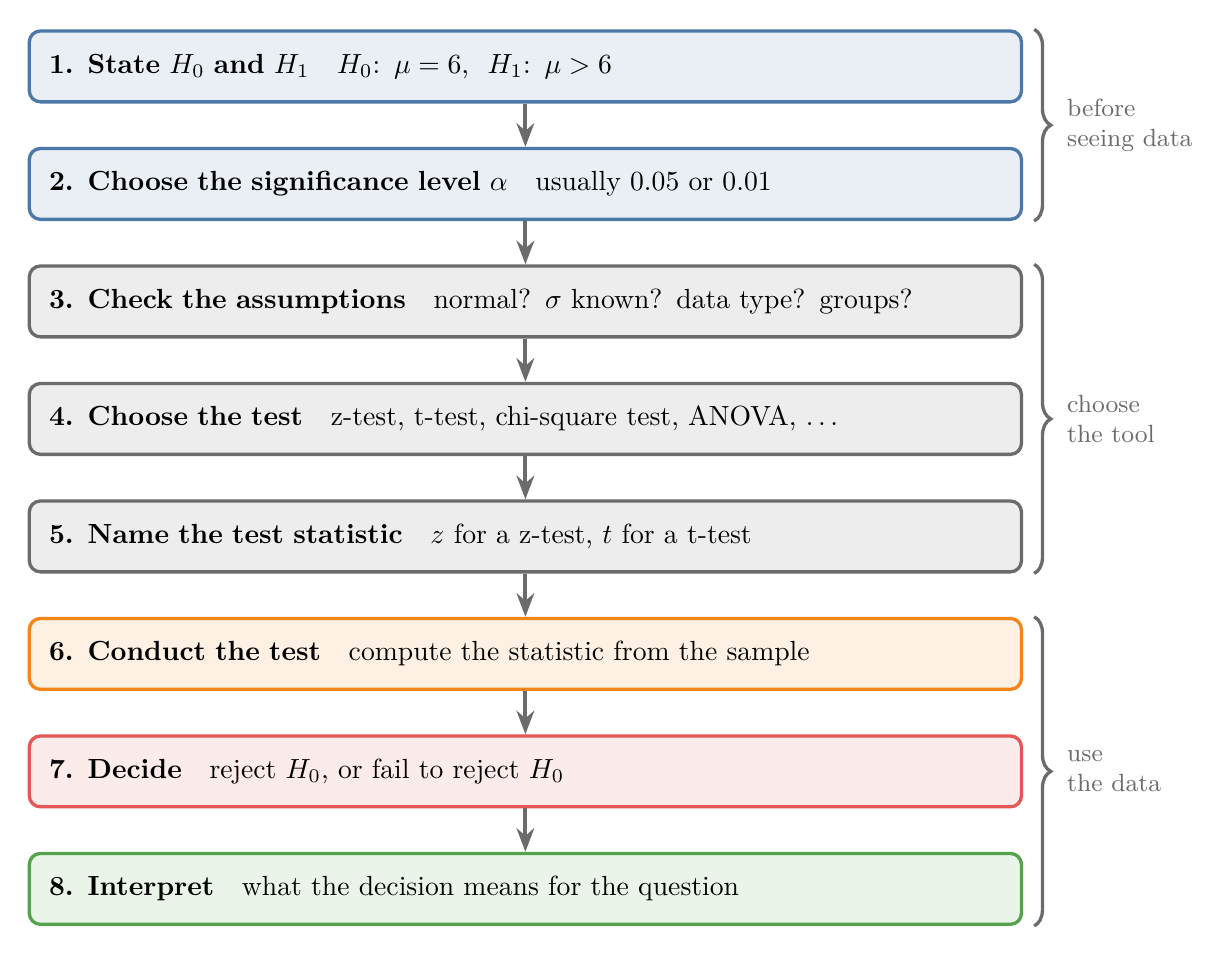
\begin{tikzpicture}[node distance=0.55cm]
  \tikzset{step/.style={box=#1, minimum width=12.6cm, text width=12.1cm, align=left, minimum height=0.9cm, inner sep=5pt}}
  \node[step=cblue] (s1) {\textbf{1. State $H_0$ and $H_1$}\quad $H_0$: $\mu = 6$, \ $H_1$: $\mu > 6$};
  \node[step=cblue, below=of s1] (s2) {\textbf{2. Choose the significance level $\alpha$}\quad usually 0.05 or 0.01};
  \node[step=cgrey, below=of s2] (s3) {\textbf{3. Check the assumptions}\quad normal? $\sigma$ known? data type? groups?};
  \node[step=cgrey, below=of s3] (s4) {\textbf{4. Choose the test}\quad z-test, t-test, chi-square test, ANOVA, \dots};
  \node[step=cgrey, below=of s4] (s5) {\textbf{5. Name the test statistic}\quad $z$ for a z-test, $t$ for a t-test};
  \node[step=corange, below=of s5] (s6) {\textbf{6. Conduct the test}\quad compute the statistic from the sample};
  \node[step=cred, below=of s6] (s7) {\textbf{7. Decide}\quad reject $H_0$, or fail to reject $H_0$};
  \node[step=cgreen, below=of s7] (s8) {\textbf{8. Interpret}\quad what the decision means for the question};
  \foreach \a/\b in {s1/s2, s2/s3, s3/s4, s4/s5, s5/s6, s6/s7, s7/s8} \draw[arrow] (\a) -- (\b);
  \draw[decorate, decoration={brace, amplitude=6pt}, draw=cgrey] ([xshift=4pt]s1.north east) -- ([xshift=4pt]s2.south east)
    node[midway, right=8pt, note, align=left] {before\\ seeing data};
  \draw[decorate, decoration={brace, amplitude=6pt}, draw=cgrey] ([xshift=4pt]s3.north east) -- ([xshift=4pt]s5.south east)
    node[midway, right=8pt, note, align=left] {choose\\ the tool};
  \draw[decorate, decoration={brace, amplitude=6pt}, draw=cgrey] ([xshift=4pt]s6.north east) -- ([xshift=4pt]s8.south east)
    node[midway, right=8pt, note, align=left] {use\\ the data};
\end{tikzpicture}
\end{document}
